\section{Person Discovery challenge}
\label{sec:challenge}


The goal of this challenge is to address the indexing of people in archives under real-world conditions when no
 pre-existing labels or biometric models exist.

\mypartitle{Task overview.} Participants are provided with a collection of TV broadcast recordings pre-segmented into shots.
Each shot $s \in \shots$ has to be automatically tagged with the names of people both speaking and appearing at the same time during the shot: this tagging algorithm is denoted by $\hypLabels : \shots \mapsto \mathcal{P}(\hypNames)$.

The list of persons is not provided \emph{a priori}, and person biometric models (neither voice nor face) can not be trained on external data. 
The only way to identify a person is by finding their name $n \in \hypNames$ in the audio (\emph{e.g.} using ASR) or visual (\emph{e.g.} using OCR) streams and associating them to the correct person (Fig. \ref{fig:evidence}). %This makes the task completely unsupervised (\emph{i.e.} using algorithms not relying on pre-existing labels or biometric models). 
%Because person names are detected and transcribed automatically, they may contain transcription errors to a certain extent (more on that later in Section~\ref{sec:metric}). 
We denote by $\refNames$ the set of all possible person names in the universe, correctly formatted as \texttt{firstname\_lastname} -- while $\hypNames$ is the set of hypothesized names.

\begin{figure}[tb]
 \centering
 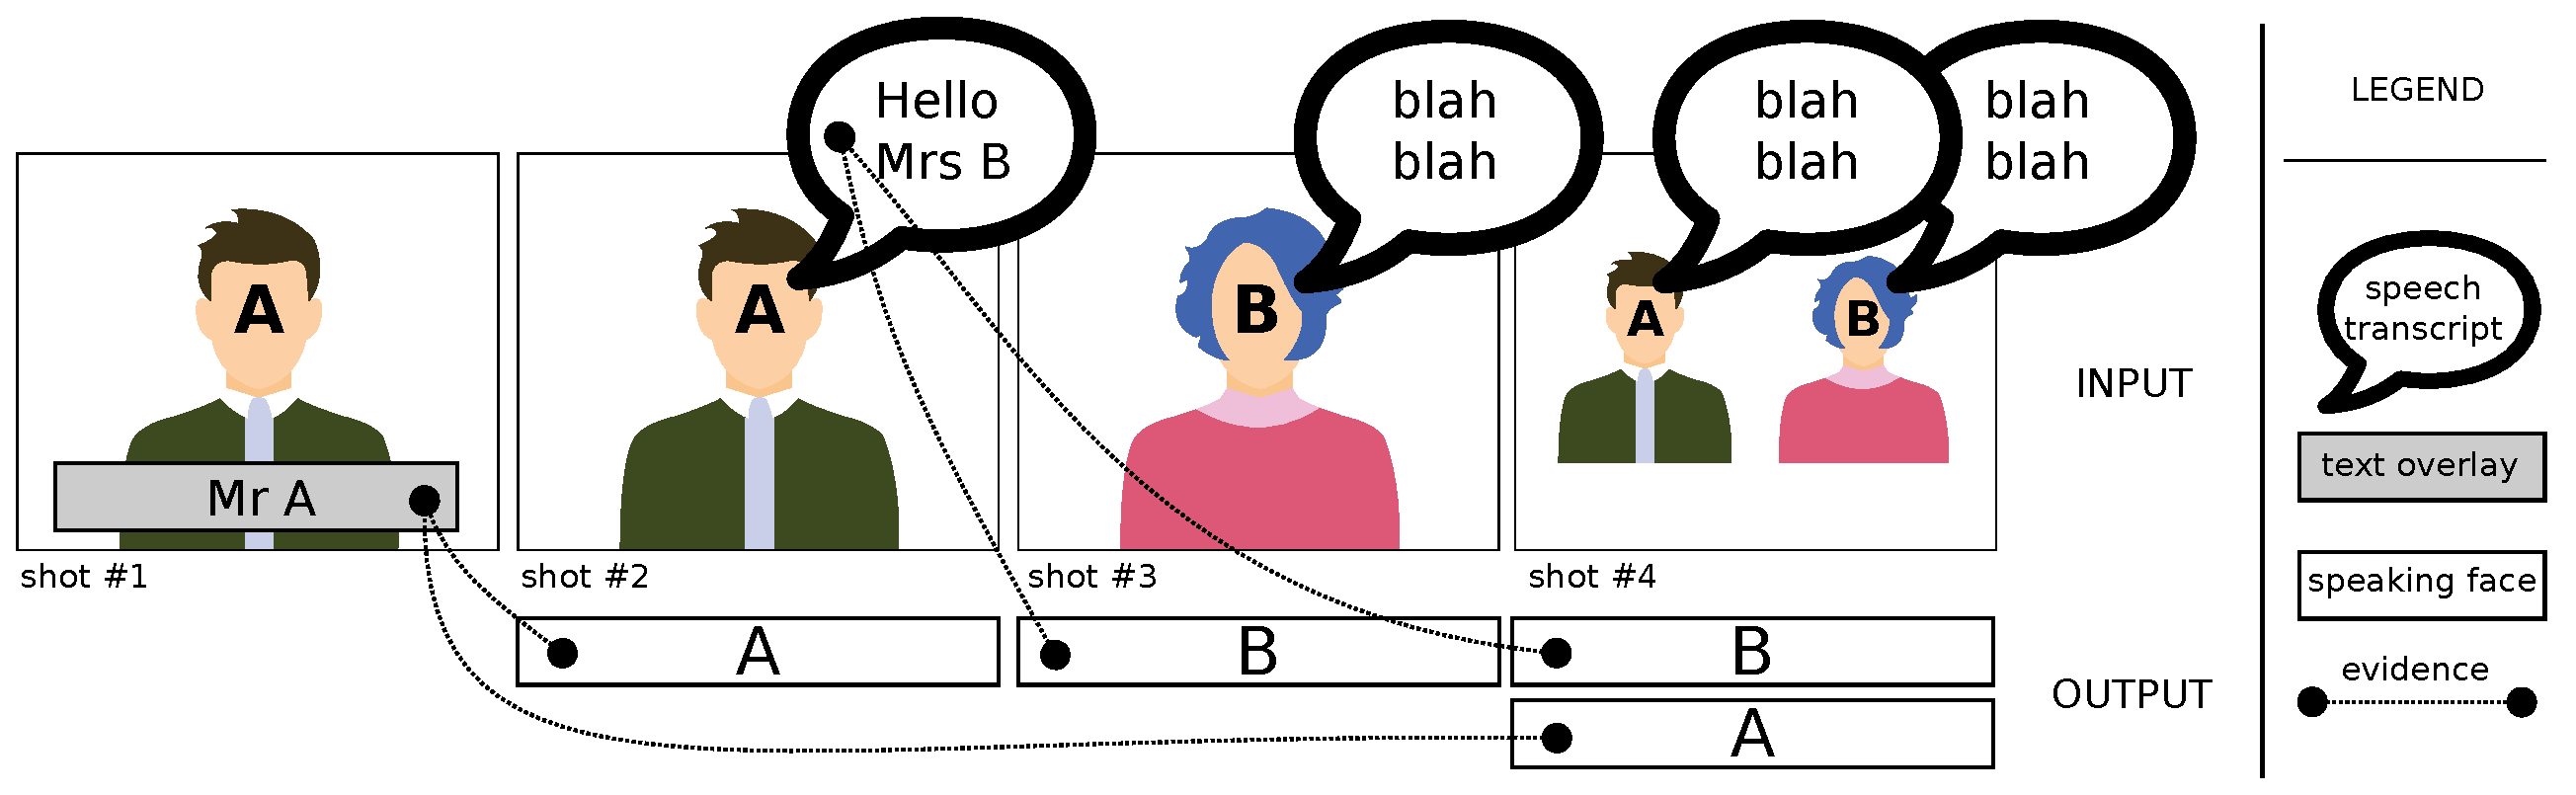
\includegraphics[width=1.\linewidth]{evidence.pdf}
\vspace*{-5mm}
 \caption{For each shot, participants have to return the names of every speaking face. An evidence is also returned for annotation process.}
\vspace*{-3mm}
 \label{fig:evidence}
\end{figure}

\mypartitle{Datasets and annotation.} The test set is divided into three sets: INA, DW and 3/24. The INA dataset contains a full week of broadcast for 2 TV french channels (total duration of 90 hours). The DW dataset~\cite{EUMSSI} is composed of video downloaded from the Deutsche Welle website, in English and German for a total duration of 50 hours. The last dataset contains 13 hours of broadcast from the 3/24 Catalan TV news channel. 

Each shot has been tagged with the names of people who appear and speak within that shot using the followign approach.
%
From all participant submissions to the challenge, a set of hypotheses were generated for each shot. 
Then participants also engaged in an interactive annotation process.
Detected names were first annotated with  thumbnails which were then used to verify whether people appeared and talked in a particular shot. 
This annotation process yielded 3431 shots with 619 identities annotated (see Tab. \ref{tab:stats} for details).

\begin{table}[tb]
\centering
\caption{Number of identities and corresponding shots where people appear and speak in each set of the corpus.}
\vspace*{-2mm}
\begin{tabular}{c|c|c|c|c|}
\cline{2-5}
    						   		& DW  	& INA 	& 3/24  & Total\\ \hline
 \multicolumn{1}{|c|}{\# shots} 		& 950	& 2250  & 231 & 3431\\ \hline

 \multicolumn{1}{|c|}{\# identities} 	& 344	& 232   & 44 & 619 \\ \hline
								
\end{tabular}
%
\vspace*{-5mm}
\label{tab:stats}
\end{table}



\mypartitle{Metrics.} The task is evaluated indirectly as an information retrieval task. %, using the following principle:
%
For each query $q \in \queries \subset \refNames$ (\texttt{first\-name\_lastname}), returned shots are first sorted by the edit distance between the hypothesized person name and the query $q$ and then by confidence scores.
The Average precision $\text{AP}(q)$ is then computed based on the list of relevant shots (according to the groundtruth) and the sorted list of shots. Finally, the Mean Average Precision is computed as follows:
\begin{align}
            \text{MAP} & = \frac{1}{|\queries|} \sum_{q \in \queries} \text{AP}(q) \nonumber
\end{align}

\mypartitle{Video OCR-NER}. As the task we aim at is fully unsupervised, 
the names of people have to be found in the audio  or visual streams.
%
%Person identities can be retrieved either from speech transcripts or from overlaid person names commonly used to introduce the current speaker. 
%
Person identification from automatic ASR transcripts usually deteriorates performance. 
Meanwhile, video text can be reliably extracted using OCR, and names of people appearing in the video 
can be relatively well distinguished in OCR outputs and 
be more easily  associated with people in the video than 
veryfing when whether pronounced names in ASR transcripts refer to people visible in the video. 
Thus, in this work we use only names coming from OCR segments.

For  OCR recognition, we relied on the approaches described in \cite{chen-pr04}.
% for text recognition in videos.
%and on \cite{daddaoua:ICDAR:05} for text recognition and indexing.
%
In brief, first the video is preprocessed with a motion filtering to reduce false alarms, 
and individual frames are processed to localize the text regions.
%
%As compared to printed documents, OCR in TV news videos encounters several challenges: low resolution of text regions, sequence of different texts continuously displayed, or small amount of text to be recognized etc.
%
Then, multiple image segmentations of the same text region are decoded, and all results are compared and 
aggregated over time to produce several hypotheses. 
%Due to the long running time, only the lower half of the videos are processed.
%
The best hypothesis is used to extract people names for identification. Then MITIE open library\footnote{\url{https://github.com/mit-nlp/MITIE}} is used to identify person names from texts. 
%
%However, detecting names for identification can be more challenging due to several factors: (a) OCR text are often not sentences but short phrases, (b) names come from various languages, and (c) there are names of editorial staff who do not appear within the video, thus are not useful for identification such as cameramen or editors.
%
To improve the raw MITIE results, a rule-based step identifies names not corresponding to introduced people (e.g. editorial staff,  
based on their roles like  cameraman or writer) since they  do not appear within the video.





\section{Overview of our approaches}
\label{sec:overview}

Conventional approaches for person recognition rely on face and/or voice biometric models.
Thus, a very large amount of trained models is needed to cover only a decent percentage of all the people in
TV shows.
%
In addition, it is not always possible to predict which people will be the most important to find in the future.
%
To solve these problems, detected people names are assigned to faces and voices following the basic principle 
that occurrences with similar faces and voices should have the same name.
%
Below, we briefly introduce the 3 different paradigms used in of this paper  to solve the task,
which have different characteristics (generative vs. discriminative models, pairwise verification vs. global optimization, etc..), 
while later sections provides more details about them.
%

\mypartitle{Clustering-based naming (CBN).} This is the most common approach. Face/speech tracks are first aggregated into homogeneous clusters according to person identities. Then each cluster is tagged with the most probable person name (Fig.\ref{fig:cbn}). 
This approach heavily depends on the  clustering quality and granularity: 
a large numer of clusters can significantly reduce the 
indexing recall, while a to small number may produce false alarms and affect the indexing precision.


\mypartitle{Verification-based naming (VBN).} To overcome the weakness of CBN, 
VBN puts higher priority on detected names, and proceed in two main steps (Fig.~\ref{fig:vbn}).
%
A person enrolment step relying on face/speech tracks reliably associated with OCR names, 
and a verification step on all other face/speech segments, which implictly ranks them according to the identity.


\mypartitle{Graph-based naming (GBN).} 
VBN propagates names based on a one-one distance while in CBN, all the distances are globally considered. 
Graph-based naming is thus proposed as an hybrid approach between them.
%
A graph is built using  face/speech tracks as a nodes and AV similarity between nodes as edge weights. 
As in VBN, some nodes are initially tagged with the names, and this information is then propagated along the edges 
within the graph (Fig.~\ref{fig:gbn}).


\endinput
